% =========================================================
% DIAGRAMA: Arquitectura general del sistema
% Archivo imagen: Ilustraciones/arch_general.png
%
% QUÉ DIBUJAR EN DRAW.IO:
%   Vista de bloques con 3 nodos principales y las capas de protocolo entre ellos.
%
%   ┌──────────────────┐     CAN Bus 500kbps      ┌──────────────────────┐
%   │  Arduino MKR     │ ◄──────────────────────► │  Raspberry Pi        │
%   │  + CAN Shield    │    ISO 11898 (física)     │                      │
%   │                  │    ISO 15765-2 (ISO-TP)   │  Python 3            │
%   │  ECU Simulator   │    SAE J1979 (OBD-II)    │  ├─ IsoTpTransport   │
%   │  ├─ Mode 01/03   │                           │  ├─ DiagnosticSession│
%   │  ├─ Mode 04/09   │                           │  ├─ BleGattServer    │
%   │  ├─ ISO-TP SF/FF │                           │  └─ SqliteLogger     │
%   │  └─ CAN Noise    │                           │                      │
%   └──────────────────┘                           │  SQLite diagnostics.db│
%                                                  └──────────┬───────────┘
%                                                             │
%                                                    BLE 2.4 GHz
%                                                    GATT / NUS
%                                                    JSON over NUS
%                                                             │
%                                              ┌──────────────▼───────────┐
%                                              │  App Móvil               │
%                                              │  React Native + Expo     │
%                                              │  ├─ ConnectionScreen     │
%                                              │  ├─ DashboardScreen      │
%                                              │  ├─ DtcScreen            │
%                                              │  ├─ LogsScreen           │
%                                              │  └─ ConsoleScreen        │
%                                              │  Zustand state stores    │
%                                              └──────────────────────────┘
%
%   Junto al bus CAN: TX: 0x7E0 | RX: 0x7E8 | 500 kbps
%   Junto al BLE: NUS UUID: 6E400001-... (nombre: diag_tool) | MTU servidor 240 / app 128 bytes
%   Botones D5 (ignición) y D4 (DTC fault) en Arduino
%   Pantallas app (tabs): Panel, Averías, Sesiones, Consola, Ajustes (+ conexión por modal)
%   ECU también responde UDS: 0x10 (DiagnosticSessionControl) y 0x22 (ReadDataByIdentifier)
%   Ruido de sensores y tramas de difusión: opcionales, desactivados por defecto
%   Leyenda de colores: Rojo=física, Naranja=transporte, Verde=aplicación
% =========================================================
% TODO draw.io: dibujar arquitectura 3 nodos (Arduino ↔ CAN ↔ RPi ↔ BLE ↔ App) y exportar como arch_general.png
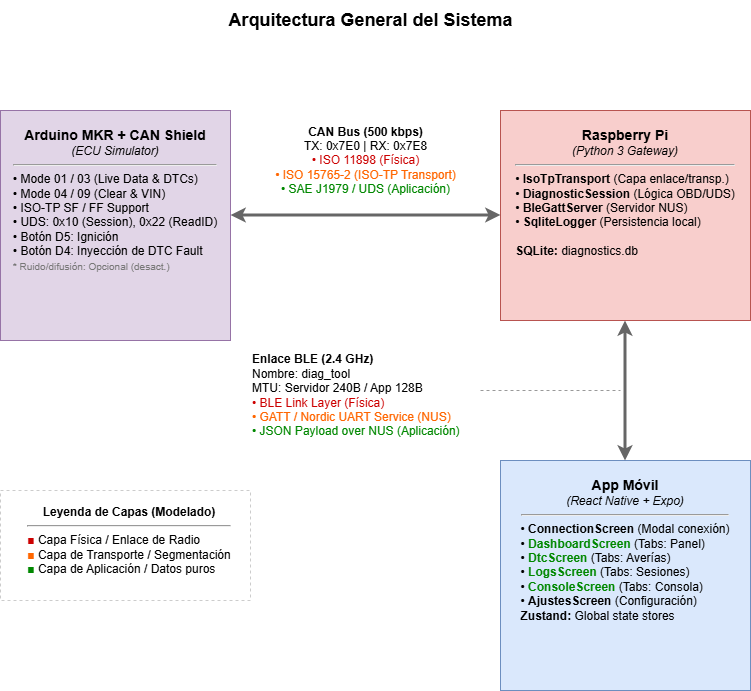
\includegraphics[width=\textwidth]{Ilustraciones/arch_general.png}
